% easychair.tex,v 3.4 2016/10/19

%\documentclass{easychair}
\documentclass[EPiC]{easychair}
%\documentclass[debug]{easychair}
%\documentclass[verbose]{easychair}
%\documentclass[notimes]{easychair}
%\documentclass[withtimes]{easychair}
%\documentclass[a4paper]{easychair}
%\documentclass[letterpaper]{easychair}
\usepackage[defaultlines=4,all]{nowidow}
\usepackage{doc}
\usepackage{subfigure}
\usepackage{tabularx}
\usepackage{booktabs}
\usepackage{framed}

%\usepackage{showframe}

% use this if you have a long article and want to create an index
% \usepackage{makeidx}

% In order to save space or manage large tables or figures in a
% landcape-like text, you can use the rotating and pdflscape
% packages. Uncomment the desired from the below.
%
% \usepackage{rotating}
% \usepackage{pdflscape}

% Some of our commands for this guide.
%
\newcommand{\easychair}{\textsf{easychair}}
\newcommand{\miktex}{MiK{\TeX}}
\newcommand{\texniccenter}{{\TeX}nicCenter}
\newcommand{\makefile}{\texttt{Makefile}}
\newcommand{\latexeditor}{LEd}

\newcommand{\ques}[1]{\textcolor{red}{#1}}

%\makeindex

%% Front Matter
%%
% Regular title as in the article class.
%
\title{ARCH-COMP18 Category Report:\\ Continuous and Hybrid Systems with Nonlinear Dynamics}

% Authors are joined by \and. Their affiliations are given by \inst, which indexes
% into the list defined using \institute
%
\author{
 Fabian Immler\inst{1}
 \and
 Matthias Althoff\inst{1}
 \and
 Xin Chen\inst{2}
\and
 Chuchu Fan\inst{3}
 \and
 Goran Frehse\inst{4}
 \and
%  Ariful Islam
%  \and 
 Niklas Kochdumper\inst{1}
 \and
 Yangge Li\inst{3}
  \and
 Sayan Mitra\inst{3}
 \and
 Mahendra Singh Tomar\inst{1}
 \and
 Majid Zamani\inst{1}
 }

\institute{
  Technische Universit\"at M\"unchen, 
  Munich, Germany\\
  \email{\{althoff,immler\}@in.tum.de,\{niklas.kochdumper,mahendrasingh.tomar,zamani\}@tum.de}\\
\and  
  University of Dayton,
  Dayton, OH, United States\\
  \email{xchen4@udayton.edu}
\and
    University of Illinois at Urbana-Champaign,
    Champaign, IL, United States\\
    \email{\{mitras,cfan10,li213\}@illinois.edu}
\and
   Univ. Grenoble Alpes,
   Grenoble, France\\
   \email{goran.frehse@univ-grenoble-alpes.fr}
}

\authorrunning{Immler \emph{et al.}}
\titlerunning{ARCH-COMP18 Nonlinear Dynamics}

\begin{document}

\maketitle

\begin{abstract}
 We present the results of a friendly competition for formal verification of continuous and hybrid systems with nonlinear continuous dynamics. The friendly competition took place as part of the workshop \underline{A}pplied Ve\underline{r}ification for \underline{C}ontinuous and \underline{H}ybrid Systems (ARCH) in 2018. In this year, six tools CORA, CORA/SX, C2E2, Flow*, Isabelle/HOL, and SymReach (in alphabetic order) participated. They are applied to solve reachability analysis problems on four benchmarks problems, one of them with hybrid dynamics. We do not rank the tools based on the results, but show the current status and discover the potential advantages of different tools.
\end{abstract}

%\setcounter{tocdepth}{2}
%{\small
%\tableofcontents}


\section{Introduction}
\label{sect:introduction}

\begin{framed}
\paragraph{Disclaimer} The presented report of the ARCH friendly competition for \textit{continuous and hybrid systems with nonlinear dynamics} aims at providing a landscape of the current capabilities of verification tools. We would like to stress that each tool has unique strengths---not all of the specificities can be highlighted within a single report. To reach a consensus in what benchmarks are used, some compromises had to be made so that some tools may benefit more from the presented choice than others. The obtained results have been verified by an independent repeatability evaluation. To establish further trustworthiness of the results, the code with which the results have been obtained is publicly available at \href{https://gitlab.com/goranf/ARCH-COMP}{gitlab.com/goranf/ARCH-COMP}.
\end{framed}


In this report, we summarize the results of the second ARCH friendly competition on the reachability analysis of continuous and hybrid systems with nonlinear dynamics. Given a system defined by a nonlinear Ordinary Differential Equation (ODE) $\dot{\vec{x}} = f(\vec{x},t)$ along with an initial condition $\vec{x} \in X_0$ as well as an unsafe set $U$, we apply the participating tools to prove that there is no state reachable contained in $U$ over a bounded time horizon. The techniques for solving such a problem are usually very sensitive to not only the nonlinearity of the dynamics but also the size of the initial set. This is also one of the main reasons why most of the tools require quite a lot of computational parameters.


In this report, six tools CORA, CORA/SX, C2E2, Flow*, Isabelle/HOL, and SymReach participate in solving the safety problems defined on three continuous and one hybrid benchmark. The continuous benchmarks are the Van der Pol oscillator, the Laub-Loomis model, and a controlled quadrotor model. The hybrid benchmark models a space rendezvous.

The benchmarks are selected based on the discussions of the tool authors. Since the experimental results are produced on different platforms, we provide Section~\ref{sec:machines} for the hardware details.



%------------------------------------------------------------------------------
\section{Participating Tools}
\label{sect:tools}

\paragraph{CORA.} The tool \textit{COntinuous Reachability Analyzer} (CORA) \cite{Althoff2015a, Althoff2016a} realizes techniques for reachability analysis with a special focus on developing scalable solutions for verifying hybrid systems with nonlinear continuous dynamics and/or nonlinear differential-algebraic equations. A further focus is on considering uncertain parameters and system inputs. Due to the modular design of CORA, much functionality can be used for other purposes that require resource-efficient representations of multi-dimensional sets and operations on them. CORA is implemented as an object-oriented MATLAB code. The modular design of CORA makes it possible to use the capabilities of the various set representations for other purposes besides reachability analysis. CORA is available at \url{http://www6.in.tum.de/Main/SoftwareCORA}.

\paragraph{CORA/SX} CORA/SX is a port of the basic zonotope reachability algorithm from the CORA Matlab toolbox to SpaceEx. There are some differences between CORA and CORA/SX. We believe they have only a minor effect on the results in this report, and we will summarize them briefly. CORA/SX varies slightly in that some matrix computations (which approximate the input over one time step) use SpaceEx code instead of an overapproximation that is based on intervals. CORA/SX uses its own proprietary symbolic differentiation to compute the Jacobian and Hessian matrices. Affine arithmetic based on the library AAFlib \cite{grabowski2008analog} is used to obtain interval bounds on the linearization error.

\paragraph{C2E2.}
C2E2 (Compare-Execute-Check-Engine) \cite{c2e2_2,c2e2_1} is a tool for verifying bounded-time invariant properties for hybrid system with both linear or nonlinear dynamics,
and discrete transitions with guards and resets. The tool implements a \textit{simulation-based approach} for overapproximating the reachable states. The input hybrid automata and the unsafe set has to be represented in an XML format. The new version of C2E2 used for these experiments (to be released in Fall 2018) comes with a model editor that can compose hybrid automata and a built-in plotter. C2E2 and related publications are available from~\url{https://publish.illinois.edu/c2e2-tool/}.

\paragraph{Flow*.} The tool Flow*~\cite{Chen+/2013/flowstar} uses an adapted Taylor Model (TM) integration method to compute reachable set overapproximations for nonlinear continuous and hybrid systems. Similar to the original method proposed in~\cite{Berz+Makino/1998/Verified}, an ODE solution, i.e., a function over the initial set as well as the time variable, over a bounded time interval is overapproximated by a TM in Flow*, and it therefore forms an overapproximation of the reachable set there. We also call this TM a TM flowpipe. For the discrete jumps of hybrid systems, Flow* uses the techniques of domain contraction and range overapproximation to compute flowpipe/guard intersections~\cite{Chen+/2012/taylor_models}, and then aggregates them by a box or parallelotope. Besides, in order to reduce the accumulation of overestimation during an integration job, the tool can symbolically represent the remainders of the previous $N$ flowpipes for some $N > 0$ (see~\cite{Chen+Sankaranarayanan/2016/decomposed}). In order to produce guaranteed results, the tool represents reals by their interval enclosures such that all roundoff errors are taken into account. In the future, we plan to improve the estimation of roundoff errors so as to make the tool more numerically stable. Flow* is available at \url{flowstar.org}.


\paragraph{Isabelle/HOL-ODE-Numerics.}
HOL-ODE-Numerics~\cite{Immler2015-TACAS,ODE-AFP} is a collection of rigorous numerical algorithms for continuous systems. It is based on Runge-Kutta methods implemented with affine arithmetic. 
The distinctive feature is that all algorithms are formally verified in the interactive
theorem prover Isabelle/HOL: everything from single roundoff errors to the global approximation
scheme is proved correct with respect to a formalization of ODEs in Isabelle/HOL.
The resulting code is therefore highly trustworthy.
It does, however, not feature many optimizations or the most sophisticated algorithms. We therefore
do not expect competitive performance figures. Nevertheless, the tool should exhibit reasonable
performance: it should scale (modulo possibly large constant factors) like ``regular'' tools
implementing similar algorithms. Isabelle/HOL is available at \url{https://isabelle.in.tum.de}, HOL-ODE-Numerics is part of the Archive of Formal Proofs \url{http://isa-afp.org/entries/Ordinary_Differential_Equations.shtml}.

\paragraph{SymReach.}
SymReach is a tool (under development) for the computation of an overapproximation of the reachable set of continuous time nonlinear systems. It is a C++ implementation of the procedure \cite{Althoff/2010/phd, Althoff2011a} that is also included in CORA, with the hope that computation time may come out to be smaller. It utilizes on-the-fly linearization using first order Taylor series and its Lagrange remainder. To compute the reachable set for each step, an interval called the applied error (AE) is assumed to enclose the linearization error. The computed error (CE) on the obtained tentative reachable set is then compared with the AE. The set is accepted if the CE is a subset of the AE, otherwise the initial set for the step is split into two and the process is repeated for each of the two newly created sets. SymReach is available at \url{https://github.com/mahendrasinghtomar/SymReach}.

%------------------------------------------------------------------------------

\newpage

\section{Benchmarks}
\label{sect:benchmarks}

\subsection{Van der Pol Oscillator}

\subsubsection{Model}

The Van der Pol oscillator was introduced by the Dutch physicist Balthasar van der Pol. It can be defined by the following ODE with $2$ variables.
\[
 \left\{
 \begin{array}{lcl}
  \dot{x} & = & y \\
  \dot{y} & = & y - x - x^2 y
 \end{array}
 \right.
\]
The system has a stable limit cycle however shows complicated behavior.

\subsubsection{Specification}

We consider the initial condition $x(0)\in [1.25,1.55]$, $y(0) \in [2.35,2.45]$ which is used in~\cite{Althoff/2010/phd}. The unsafe set is given by $y \geq 2.75$ for the time horizon $[0,7]$.


\subsubsection{Results}

The time costs of the participating tools on the Van der Pol oscillator benchmark are given in Table~\ref{tab:compTimes:vanderpol}, and the plots of the overapproximation sets are presented in Figure~\ref{fig:vanderpol}. We also provide the computational settings of the tools as below.

\begin{figure}[p]
\centering
\subfigure[CORA.] 
	  {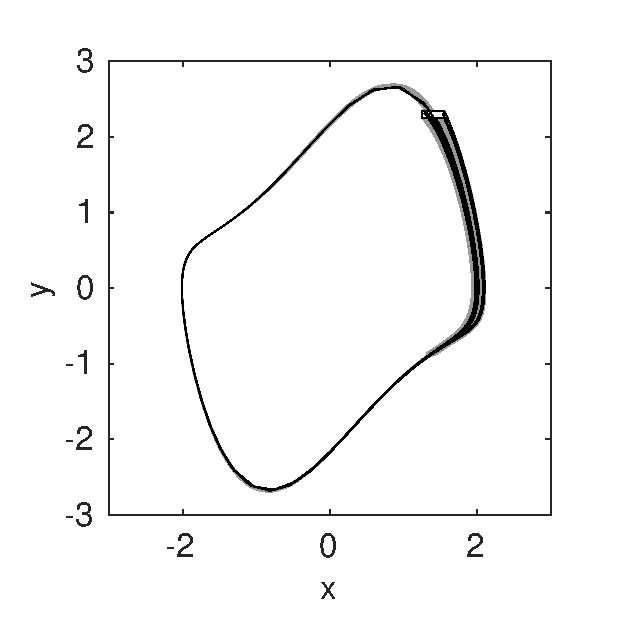
\includegraphics[width=5.5cm, height=5.5cm]{results_CORA/vanDerPol_30May2018.eps}
  \label{fig:vanderpol:CORA}}
%  \hspace{0.2in}
\subfigure[CORA/SX.] 
	  {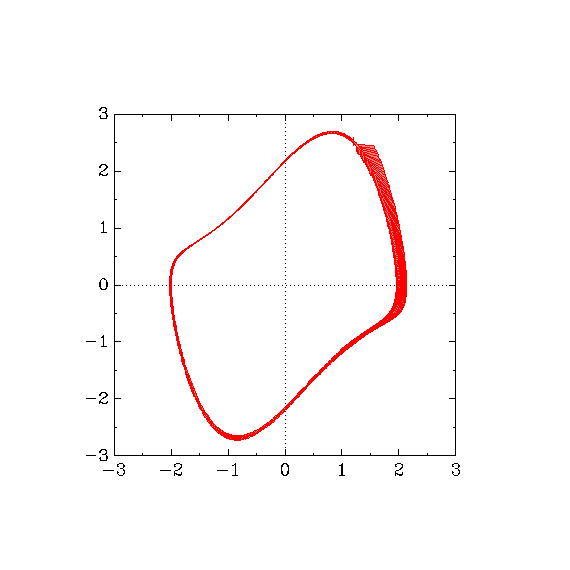
\includegraphics[width=5.5cm, height=5.5cm, trim=50 50 50 50, clip=true]{results_SpaceEx/vdp-zono.png}
  \label{fig:vanderpol:CORASX}}
%  \hspace{0.2in}
\subfigure[C2E2.] 
	  {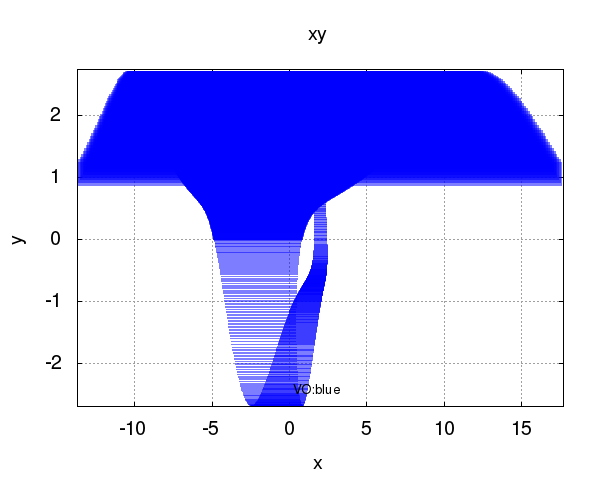
\includegraphics[width=5.5cm, height=5.5cm]{results_C2E2/vanderpol.png}
  \label{fig:vanderpol:C2E2}}
%  \hspace{0.2in}
\subfigure[Flow*.] 
	  {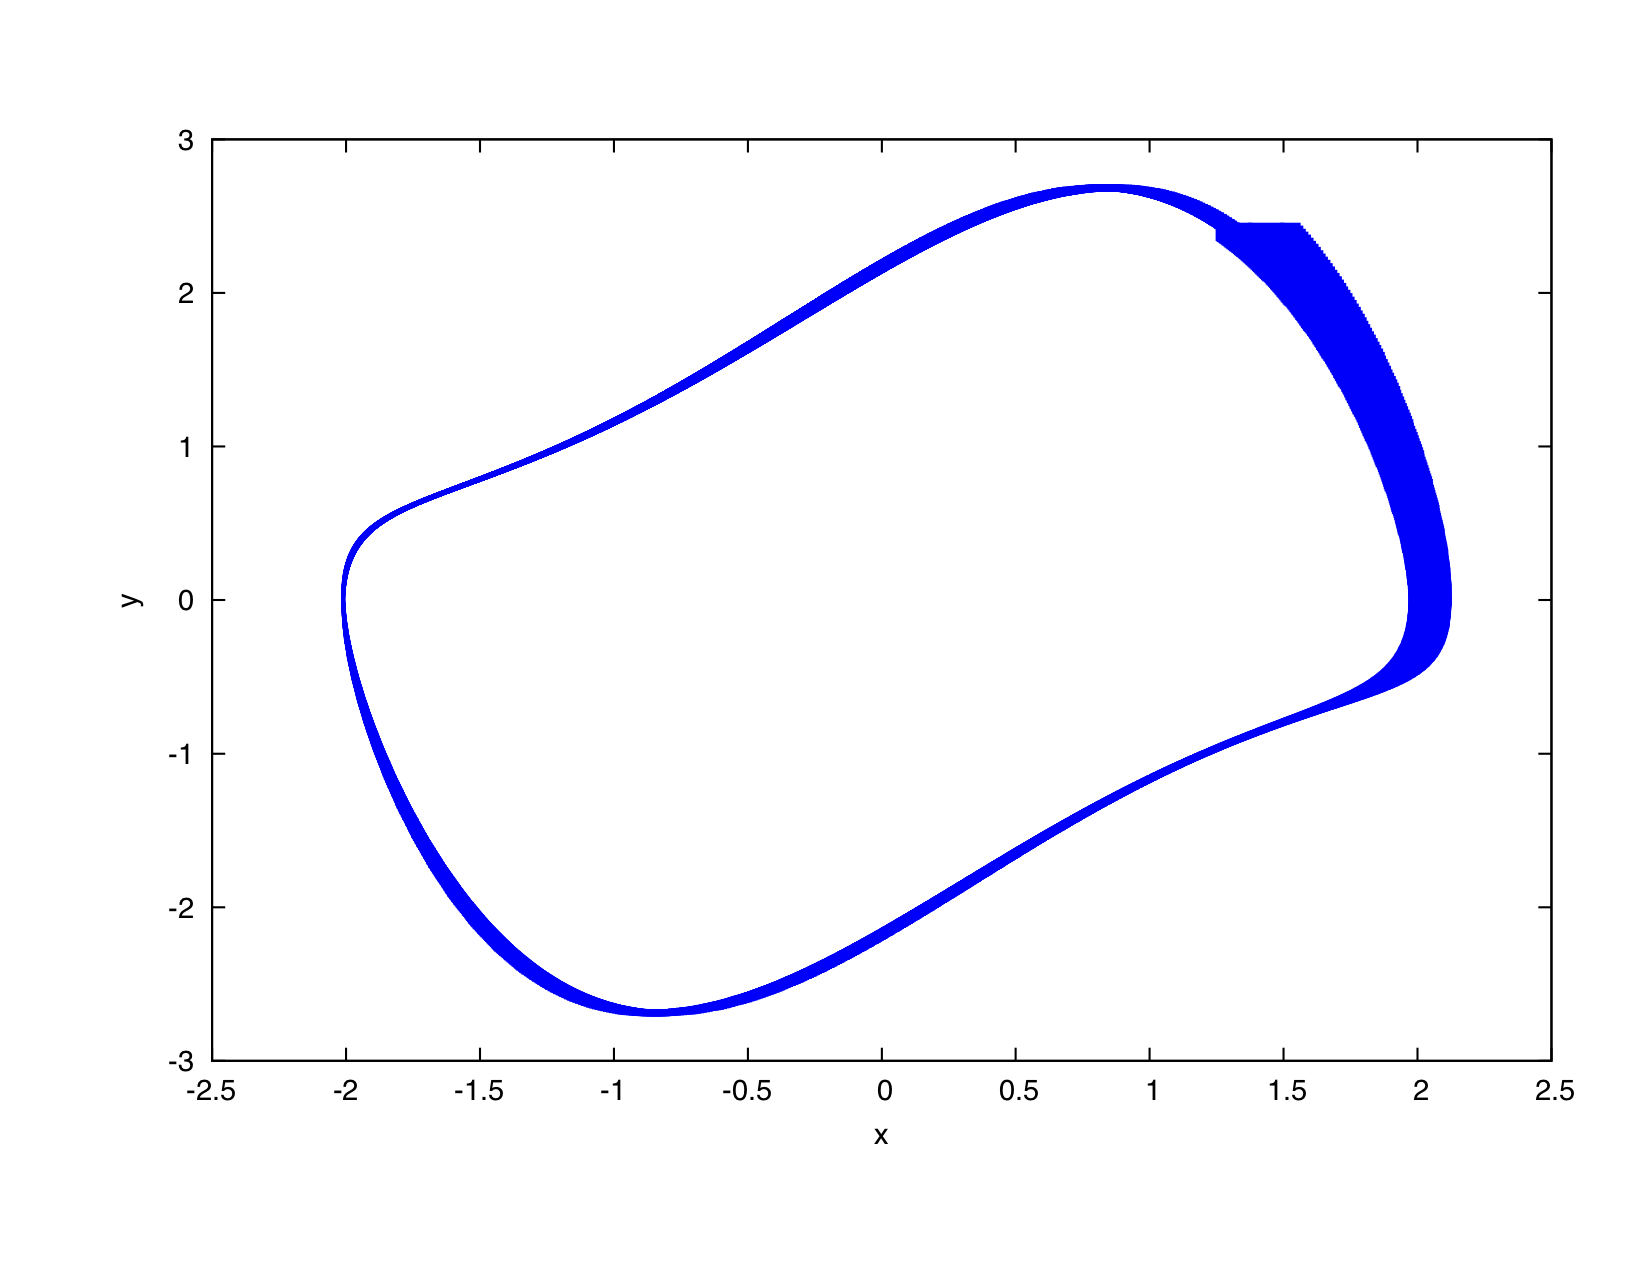
\includegraphics[width=5.5cm, height=5.5cm]{results_flowstar/vanderpol.png}
  \label{fig:vanderpol:flowstar}}
%  \hspace{0.2in}
\subfigure[Isabelle/HOL.] 
	  {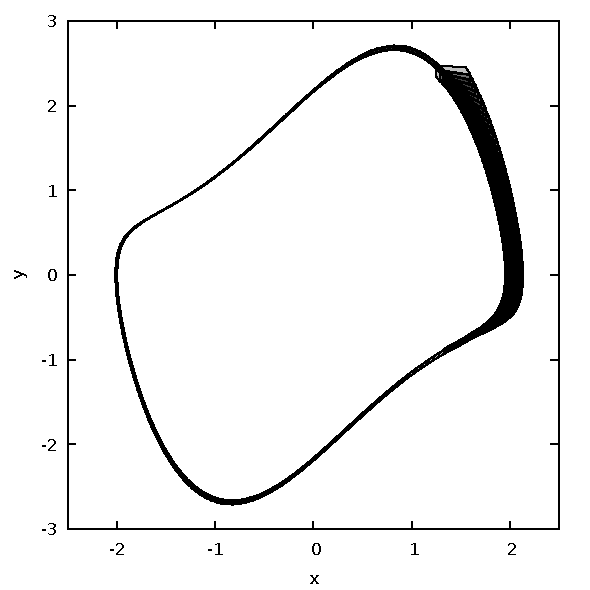
\includegraphics[width=5.5cm, height=5.5cm]{results_Isabelle/out_p1_vdp_0.pdf}
  \label{fig:vanderpol:isabelle}}
%  \hspace{0.2in}
\subfigure[SymReach.] 
	  {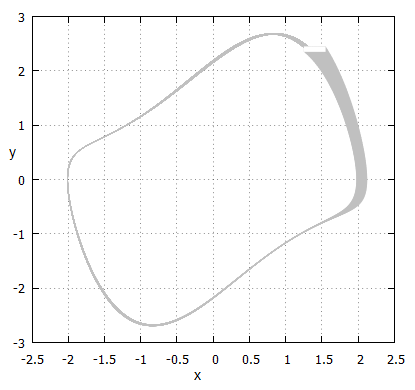
\includegraphics[width=5.5cm, height=5.5cm]{results_SymReach/vanderpol.png}
  \label{fig:vanderpol:SymReach}}
\caption{Reachable set overapproximations for the Van der Pol oscillator.}
\label{fig:vanderpol}
\end{figure}

\begin{table}[t]
	\setlength{\tabcolsep}{4pt}
	\renewcommand{\arraystretch}{1.2}
	\centering
	\caption{Results of the Van der Pol Oscillator. Details of the platforms are described in Section~\ref{sec:machines}.}\label{tab:compTimes:vanderpol}
	\begin{tabular}[c]{lccc}
	\hline
		 \textbf{tool} & \textbf{computation time in [s]} & \textbf{language} & \textbf{machine} \\
		 \hline
         CORA & $2.3$ & MATLAB & M$_{\text{CORA}}$ \\
         CORA/SX & $0.6$ & C++ & M$_{\text{SpaceEx}}$ \\
         {C2E2} & {$38.5$} & {C++} & {M$_{\text{C2E2}}$} \\
         Flow* & $1.5$ & C++ & M$_{\text{Flow*}}$ \\
         Isabelle/HOL & $1.5$ & SML & M$_{\text{Isabelle}}$ \\
         SymReach & $17.14$ & C++ & M$_{\text{SymReach}}$ \\
		 \hline
	\end{tabular}
\end{table}

\paragraph{Setting for CORA.}
CORA has introduced a pseudo invariant at $x=1.5$. Further, CORA uses the time step size $0.01$ and the zonotope order is chosen as $20$. 

\paragraph{Setting for CORA/SX.}
A pseudo invariant at $x=1.2$ was introduced manually. The time step size is $0.01$ and the zonotope order is chosen as $20$. 

\paragraph{Setting for C2E2.} C2E2 proved the safety of the model by using time step size $0.01$. The K value is chosen to be 1000. The reachtube for variable $x$ is over bloated due to the lack of constraints on variable $x$. The reachtube overapproximation is enough for proving the safety constraints on variable $y$. Note that the result for C2E2 is not optimal since C2E2 is currently been updated.

\paragraph{Setting for Flow*.}
Flow* uses the step size $0.04$, the TM order $6$, the cutoff threshold $10^{-6}$, and the precision $53$ for floating-point numbers. The TM flowpipe remainders are kept symbolically every $100$ steps. All floating-point roundoff errors are included in the overapproximations. Since there are only $2$ state variables, the tool plots a grid overapproximation for the flowpipes, see Figure~\ref{fig:vanderpol:flowstar}. The approximation quality can be better evaluated based on the remainder size of the last TM flowpipe (see~\cite{Chen/2015/phd}). In this task, the overapproximation error for the last flowpipe is bounded by only $0.01214$.


\paragraph{Setting for Isabelle/HOL.}
Maximum Zonotope order is set to $20$, Reachability analysis is carried out with an (absolute and relative) error tolerance of $2^{-14}$. A pseudo-invariant is added at $x=1.5$. 

\paragraph{Setting for SymReach}
Step size is set to $0.01$, zonotope order limited to $20$, $L_{max} = 0.01$ (if CE $ \not\subset [-L_{max},L_{max}]$ then set split).


\subsection{Laub-Loomis Benchmark}

\subsubsection{Model}

The Laub-Loomis model is presented in~\cite{Laub+Loomis/1998/oscillator} for studying a class of enzymatic activities. The dynamics can be defined by the following ODE with $7$ variables.
\[
\left\{
\begin{array}{lcl}
 \dot{x}_1 & = & 1.4 x_3 - 0.9 x_1 \\
 \dot{x}_2 & = & 2.5 x_5 - 1.5 x_2 \\
 \dot{x}_3 & = & 0.6 x_7 - 0.8 x_2 x_3 \\
 \dot{x}_4 & = & 2 - 1.3 x_3 x_4 \\
 \dot{x}_5 & = & 0.7 x_1 - x_4 x_5 \\
 \dot{x}_6 & = & 0.3 x_1 - 3.1 x_6 \\
 \dot{x}_7 & = & 1.8 x_6 - 1.5 x_2 x_7
\end{array}
\right.
\]
The system is asymptotically stable and the equilibrium is the origin.


\subsubsection{Specification}

The initial sets are defined according to the one used in~\cite{Testylier+/2013/NLTOOLBOX}. They are boxes centered at $x_1(0) = 1.2$, $x_2(0) = 1.05$, $x_3(0) =
1.5$, $x_4(0) = 2.4$, $x_5(0) = 1$, $x_6(0) = 0.1$, $x_7(0) = 0.45$. The width of the initial set is vital to the difficulty of the reachability analysis job. The larger the initial set the harder the reachability analysis. In the paper, we consider the initial box of the radius $W = 0.01$ and $W = 0.1$, i.e., the range of the box in the $i$th dimension is defined by the interval $[x_i(0)-W, x_i(0)+W]$. For the smaller initial box, we consider the unsafe region defined by $x_4 \geq 4.5$, while for the larger one, the unsafe set is defined by $x_4 \geq 5$. The time horizon for both of the cases is $[0,20]$.


\subsubsection{Results}

The computation results of the tools are given in Table~\ref{tab:compTimes:laubloomis}. It can be seen that enlarging the initial set size can greatly make the reachability analysis task harder. The tool settings are given as below. Since the safety condition is only related to the variable $x_4$, we present the plots of projections of the overapproximations in the $t$-$x_4$ plane such that $t$ is the time variable. Figure~\ref{fig:laubloomis:1} shows the results for the smaller initial set ($W = 0.01$), Figure~\ref{fig:laubloomis:2} for the larger one ($W = 0.1$). 

\begin{table}[t]
	\setlength{\tabcolsep}{4pt}
	\renewcommand{\arraystretch}{1.2}
	\centering
	\caption{Results of the Laub-Loomis model. Details of the platforms are described in Section~\ref{sec:machines}.}
	\begin{tabular}[c]{lcccc}
	\hline
		 & \multicolumn{2}{c}{\textbf{computation time in [s]}} & \multicolumn{2}{c}{\textbf{platform}} \\ \cmidrule(l){2-3} \cmidrule(l){4-5}
		 \textbf{tool} & \textbf{$W=0.01$} & \textbf{$W=0.1$} & $\textbf{language}$ & $\textbf{machine}$ \\ \hline
         CORA & $0.82$ & $63$ & MATLAB & M$_{\text{CORA}}$ \\
         CORA/SX & $0.85$ & -- & C++ & M$_{\text{SpaceEx}}$ \\
         C2E2 & {$0.12$} & {$0.67$} & {C++} & M$_{\text{C2E2}}$ \\
         Flow* & $4.5$ & $12.7$ & C++ & M$_{\text{Flow*}}$ \\
         Isabelle/HOL & $10$ & $-$ & SML & M$_{\text{Isabelle}}$ \\
         SymReach & $1.93$ & $-$ & C++ & M$_{\text{SymReach}}$ \\
		 \hline
	\end{tabular}
	\label{tab:compTimes:laubloomis}
\end{table}


\begin{figure}[p]
\centering
\subfigure[CORA] 
	  {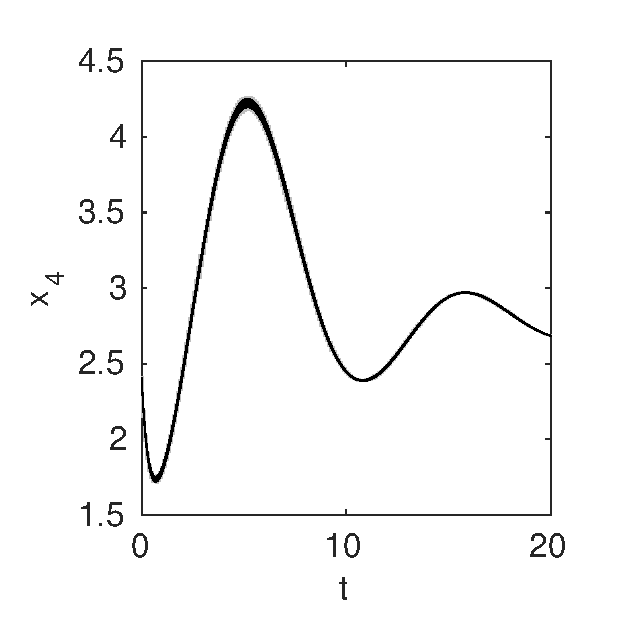
\includegraphics[width=5.5cm, height=5.5cm]{results_CORA/laubLoomis_W001_30May2018.eps}
  \label{fig:laubloomis:cora:smaller}}
  \hspace{0.2in}
\subfigure[CORA/SX] 
	  {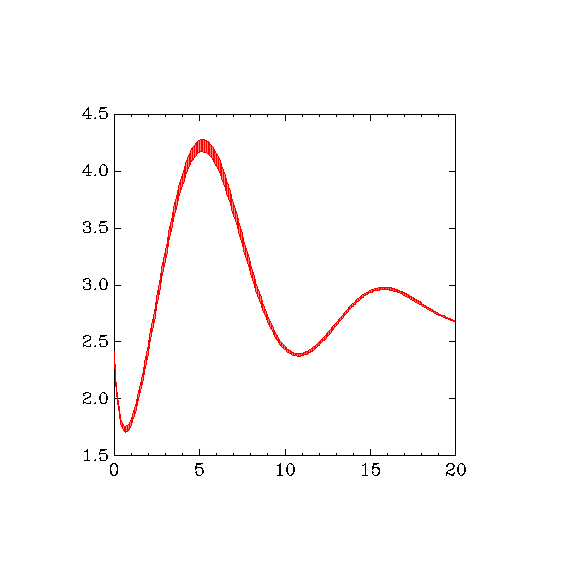
\includegraphics[width=5.5cm, height=5.5cm,trim=50 50 50 50,clip=true]{results_SpaceEx/laub_zono_0_01_plot.png}
  \label{fig:laubloomis:corasx:smaller}}\\
\subfigure[C2E2] 
	  {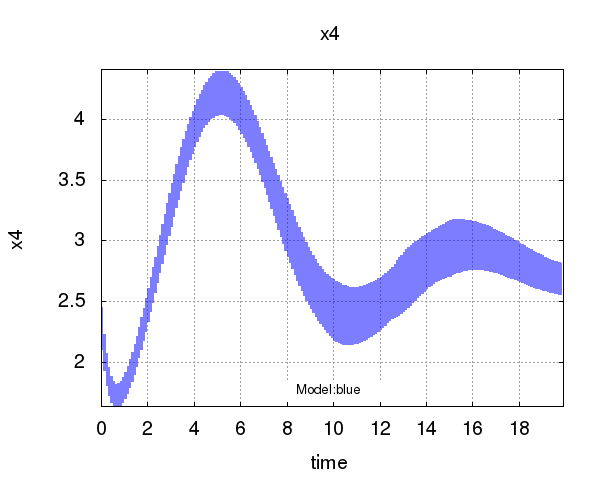
\includegraphics[width=5.5cm, height=5.5cm]{results_C2E2/laub_small.png}
  \label{fig:laubloomis:C2E2:smaller}}
  \hspace{0.2in}
\subfigure[Flow*] 
	  {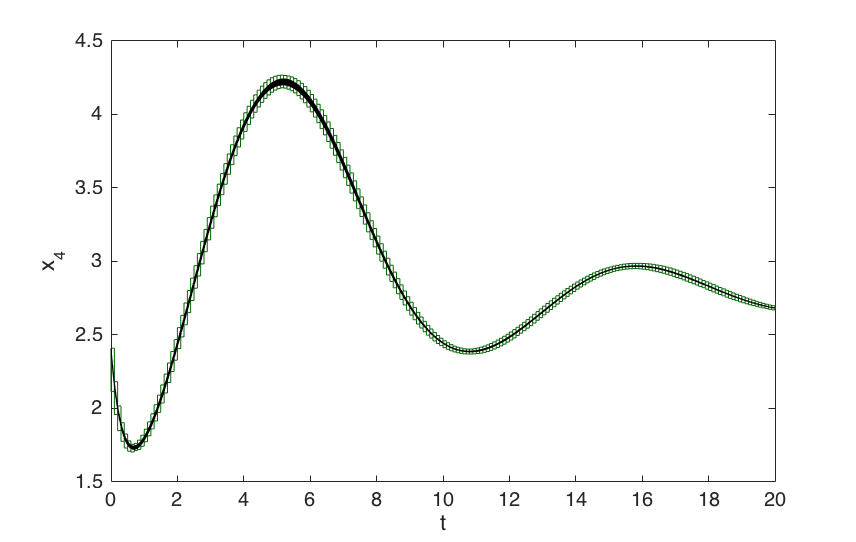
\includegraphics[width=5.5cm, height=5.5cm]{results_flowstar/laub_loomis_small.png}
  \label{fig:laubloomis:flowstar:smaller}}
  \hspace{0.2in}
\subfigure[Isabelle/HOL] 
	  {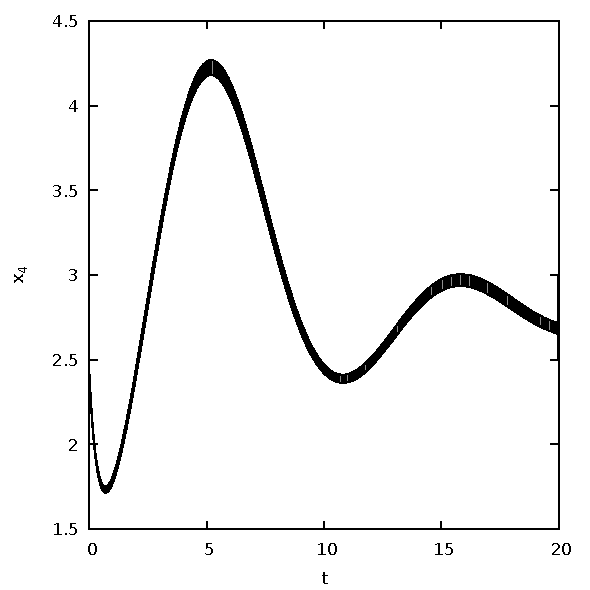
\includegraphics[width=5.5cm, height=5.5cm]{results_Isabelle/out_ll_001.pdf}
  \label{fig:laubloomis:isabelle}}
\hspace{0.2in}
\subfigure[SymReach] 
	  {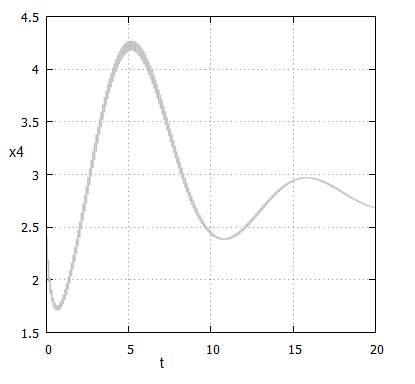
\includegraphics[width=5.5cm, height=5.5cm]{results_SymReach/laubloomisW0p02.png}
  \label{fig:laubloomis:SymReach:smaller}}
\caption{Reachable set overapproximations for the Laub-Loomis model ($W = 0.01$). CORA and Flow* show numerical simulations in black.}
\label{fig:laubloomis:1}
\end{figure}

\begin{figure}[t]
\centering
\subfigure[CORA] 
	  {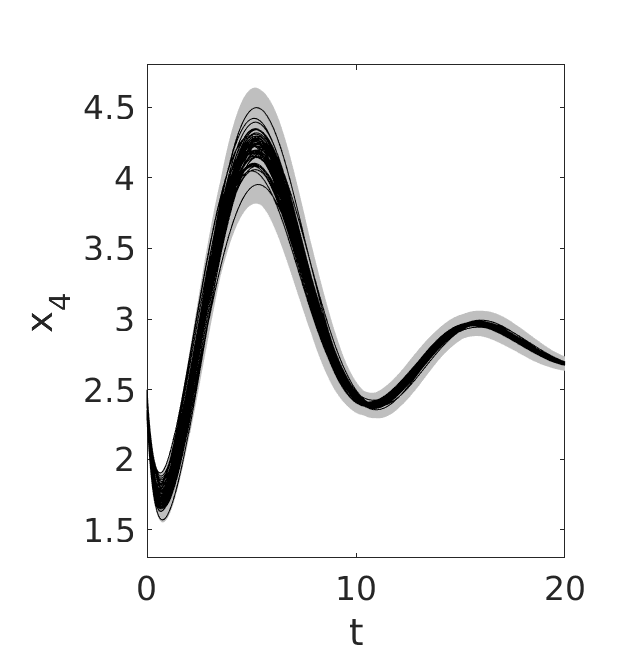
\includegraphics[width=5.5cm, height=5.5cm]{results_CORA/laubLoomis_W01_30May2018.eps}
  \label{fig:laubloomis:cora:larger}}
\subfigure[C2E2] 
	  {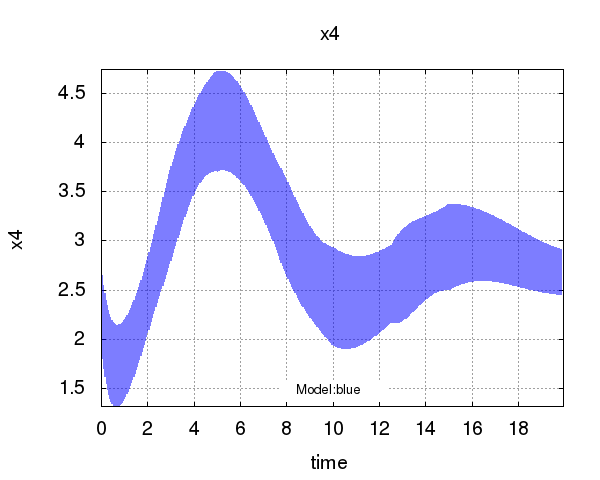
\includegraphics[width=5.5cm, height=5.5cm]{results_C2E2/laub_large.png}
  \label{fig:laubloomis:C2E2:larger}}
    \hspace{0.2in}
\subfigure[Flow*] 
	  {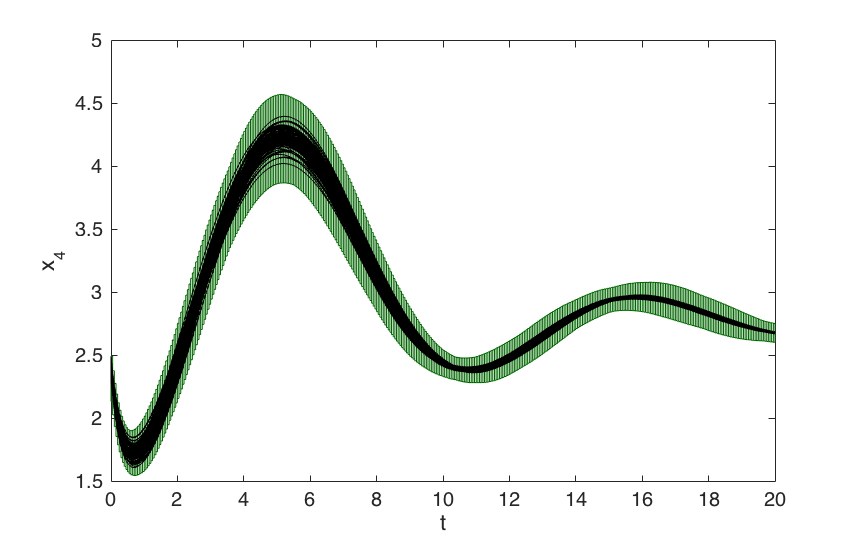
\includegraphics[width=5.5cm, height=5.5cm]{results_flowstar/laub_loomis_large.png}
  \label{fig:laubloomis:flowstar:larger}}
%\hspace{0.24in}
%\subfigure[SymReach: $W = 0.1$] 
%	  {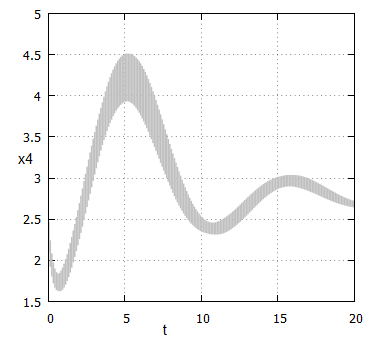
\includegraphics[width=0.45\columnwidth, height=5cm]{results_SymReach/laubloomisW0p1.png}
%  \label{fig:laubloomis:SymReach:larger}}
\caption{Reachable set overapproximations for the Laub-Loomis model ($W = 0.1$). CORA and Flow* show numerical simulations in black.}
\label{fig:laubloomis:2}
\end{figure}

\clearpage

\paragraph{Setting for CORA.}
Depending on whether the smaller or larger initial sets are used, different algorithms in CORA are applied. For the smaller initial set, the faster but less accurate algorithm presented in \cite{Althoff2008c} is executed. For the larger initial set, the more accurate but slower algorithm from \cite{Althoff2013a} is used. CORA uses a step size of $0.1$ for the small initial set and a step size of $0.05$ for the large initial set. The maximum zonotope order for both initial sets is chosen as $50$.

\paragraph{Setting for CORA/SX.}
Since CORA/SX does not currently support splitting the initial states, only the small initial set was handled. The time step is $0.1$ and the zonotope order is $50$.

\paragraph{Setting for C2E2.}
For the small initial set, C2E2 uses step size 0.1 and K value 50. For the large initial set, C2E2 uses step size 0.05 and K value 100. Note that the result for C2E2 are not optimal due to the updating of C2E2. Note that the result for C2E2 is not optimal since C2E2 is currently been updated.

\paragraph{Setting for Flow*.}
For the small initial set, Flow* uses the step size $0.1$, the TM order $4$, the cutoff threshold $10^{-7}$ and the precision $53$ for floating-point numbers. The TM flowpipe remainders are kept symbolically every $50$ steps. Besides the safety set that is defined by $x_4 \leq 4.5$, the tool even proves that $x_4 \leq 4.3$ is safe. On the other hand, for the large initial set, we use the same setting except that the stepsize is reduced to $0.05$, and the remainders are kept symbolically every $100$ steps. Besides the given safety property, the tool proves a smaller safe set which is defined by $x_4 \leq 4.6$. The plots of the flowpipes are shown in Figure~\ref{fig:laubloomis:flowstar:smaller} and~\ref{fig:laubloomis:flowstar:larger}. Notice that they are only the interval overapproximations of the flowpipes, the exact flowpipes are much more accurate, since for the small initial set, the maximum overapproximation error of the last flowpipe is only $0.01044$ which is determined by the $x_4$-dimension, while for the large initial set, the corresponding maximum error is only $0.06016$.


\paragraph{Setting for Isabelle/HOL.}
Maximum Zonotope order is set to $60$. Reachability analysis is carried out with an (absolute and relative) error tolerance of $2^{-12}$. Compared to last year, we dropped the analysis of the larger initial set, since this required many subdivisions and is too inefficient.

\paragraph{Setting for SymReach.}
Step size is set to $0.1$, zonotope order limited to $40$, $L_{max} = 0.05$. 



\subsection{Quadrotor Benchmark}

\subsubsection{Model}

We study the dynamics of a quadrotor as derived in \cite[eq. (16) - (19)]{Beard2008}. Let us first introduce the variables required to describe the model: The inertial (north) position $x_1$, the inertial (east) position $x_2$, the altitude $x_3$, the longitudinal velocity $x_4$, the lateral velocity $x_5$, the vertical velocity $x_6$, the roll angle $x_7$, the pitch angle $x_8$, the yaw angle $x_9$, the roll rate $x_{10}$, the pitch rate $x_{11}$, and the yaw rate $x_{12}$. We further require the following parameters: gravity constant $g = 9.81$ [m/s$^2$], radius of center mass $R = 0.1$ [m], distance of motors to center mass $l = 0.5$ [m], motor mass $M_{rotor} = 0.1$ [kg], center mass $M = 1$ [kg], and total mass $m = M + 4M_{rotor}$.

From the above parameters we can compute the moments of inertia as 
\begin{equation*}
\begin{split}
J_x =& \frac{2}{5} \, M \, R^2 + 2 \, l^2 \, M_{rotor}, \\
J_y =& J_x, \\
J_z =& \frac{2}{5} \, M \, R^2 + 4 \, l^2 \, M_{rotor}.
\end{split}
\end{equation*}

Finally, we can write the set of ordinary differential equations for the quadrotor according to \cite[eq. (16) - (19)]{Beard2008}:
\[
\left\{
\begin{array}{lcl}
\dot{x}_1 & = & \cos(x_8)\cos(x_9)x_4 + \Big(\sin(x_7)\sin(x_8)\cos(x_9) - \cos(x_7)\sin(x_9)\Big)x_5 \\
& & + \Big(\cos(x_7)\sin(x_8)\cos(x_9) + \sin(x_7)\sin(x_9)\Big)x_6 \\
\dot{x}_2 & = & \cos(x_8)\sin(x_9)x_4 + \Big(\sin(x_7)\sin(x_8)\sin(x_9) + \cos(x_7)\cos(x_9)\Big)x_5 \\
& & + \Big(\cos(x_7)\sin(x_8)\sin(x_9) - \sin(x_7)\cos(x_9)\Big)x_6 \\
\dot{x}_3 & = & \sin(x_8)x_4 - \sin(x_7)\cos(x_8)x_5 - \cos(x_7)\cos(x_8)x_6 \\
\dot{x}_4 & = & x_{12}x_5 - x_{11}x_6 - g\sin(x_8) \\
\dot{x}_5 & = & x_{10}x_6 - x_{12}x_4 + g\cos(x_8)\sin(x_7) \\
\dot{x}_6 & = & x_{11}x_4 - x_{10}x_5 + g\cos(x_8)\cos(x_7) - \frac{F}{m} \\
\dot{x}_7 & = & x_{10} + \sin(x_7)\tan(x_8)x_{11} + \cos(x_7)\tan(x_8)x_{12} \\
\dot{x}_8 & = & \cos(x_7)x_{11} - \sin(x_7)x_{12} \\
\dot{x}_9 & = & \frac{\sin(x_7)}{\cos(x_8)}x_{11} + \frac{\cos(x_7)}{\cos(x_8)}x_{12} \\
\dot{x}_{10} & = & \frac{J_y - J_z}{J_x}x_{11}x_{12} + \frac{1}{J_x}\tau_\phi \\
\dot{x}_{11} & = & \frac{J_z - J_x}{J_y}x_{10}x_{12} + \frac{1}{J_y}\tau_\theta \\
\dot{x}_{12} & = & \frac{J_x - J_y}{J_z}x_{10}x_{11} + \frac{1}{J_z}\tau_\psi 
\end{array}
\right.
\]

To check interesting control specifications, we stabilize the quadrotor using simple PD controllers for height, roll, and pitch. The inputs to the controller are the desired values for height, roll, and pitch $u_1$, $u_2$, and $u_3$, respectively. The equations of the controllers are
\[
\begin{array}{lcll}
F & = & m \, g - 10(x_3 - u_1) + 3x_6 \; & (\text{height control}), \\
\tau_\phi & = & -(x_7 - u_2) - x_{10} & (\text{roll control}), \\
\tau_\theta & = & -(x_8 - u_3) - x_{11} & (\text{pitch control}).
\end{array}
\]

We leave the heading uncontrolled so that we set $\tau_\psi = 0$.

\subsubsection{Specification}

The task is to change the height from $0$~[m] to $1$~[m] within $5$~[s]. A goal region $[0.98,1.02]$ of the height $x_3$ has to be reached within $5$~[s] and the height has to stay below $1.4$ for all times. After $1$~[s] the height should stay above $0.9$~[m]. The initial position of the quadrotor is uncertain in all directions within $[-0.4,0.4]$~[m] and also the velocity is uncertain within $[-0.4,0.4]$~[m/s] for all directions. All other values are initialized as $0$.

%\[
%\left\{
%\begin{array}{lcl}
% \dot{x} & = & \cos(\theta) \cos(\psi) p + (\sin(\phi) \sin(\theta) \cos(\psi) - \cos(\phi) \sin(\psi)) q + (\cos(\phi) \sin(\theta) \cos(\psi) + \sin(\phi) \sin(\psi)) r \\
% \dot{y} & = & \cos(\theta) \sin(\phi) p + (\sin(\phi) \sin(\theta) \sin(\psi) + \cos(\phi) \cos(\psi)) q + (\cos(\phi) \sin(\theta) \sin(\psi) - \sin(\phi) \cos(\psi)) r \\
% \dot{h} & = & \sin(\theta) p - \sin(\phi) \cos(\theta) q - \cos(\phi) \cos(\theta) r \\
% \dot{p} & = & w q - v r - 9.81 \sin(\theta) \\
% \dot{q} & = & u r - w p + 9.81 \cos(\theta \sin(\phi)) \\
% \dot{r} & = & v p - u q + 9.81 \cos(\theta \cos(\phi)) - 9.81 + 7.14285714285714 (h - 1) - 2.14285714285714 \, r \\
% \dot{\phi} & = & u + (\sin(\phi) \tan(\theta)) v + (\cos(\phi) \tan(\theta)) w \\
% \dot{\theta} & = & \cos(\phi) v - \sin(\phi) w \\
% \dot{\psi} & = & (\sin(\phi)/\cos(\theta)) v + (\cos(\phi)/\cos(\theta)) w \\
% \dot{u} & = & -0.92592592592593 v w - 18.51851851851852 (\phi + u) \\
% \dot{v} & = & 0.92592592592593 u w - 18.51851851851852 (\theta + v) \\
% \dot{w} & = & 0 \\
%\end{array}
%\right.
%\]

\begin{figure}[htb]
\centering
\subfigure[CORA.] 
	  {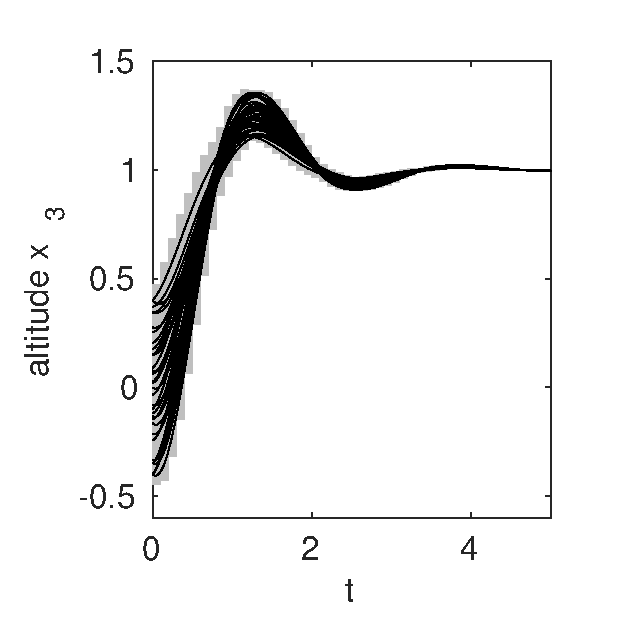
\includegraphics[width=5.5cm, height=5.5cm]{results_CORA/quadrocopterControlled_29June2018.eps}
  \label{fig:quadrotor:cora}}
  \hspace{0.2in}
\subfigure[CORA/SX.] 
	  {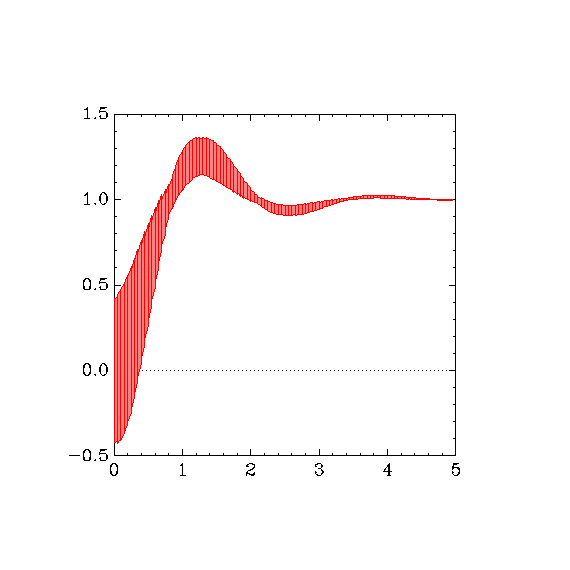
\includegraphics[width=5.5cm, height=5.5cm,trim=50 50 50 75, clip=true]{results_SpaceEx/quad_zono_plot.png}
  \label{fig:quadrotor:corasx}}
  \hspace{0.2in}
\subfigure[Flow*.] 
	  {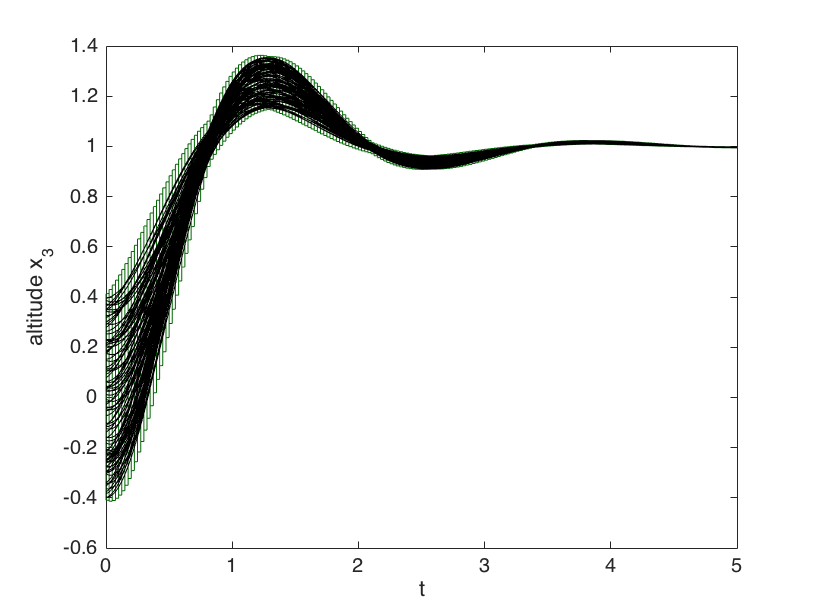
\includegraphics[width=5.5cm, height=5.5cm]{results_flowstar/quadrotor.png}
  \label{fig:quadrotor:flow*}}
\subfigure[Isabelle/HOL.] 
	  {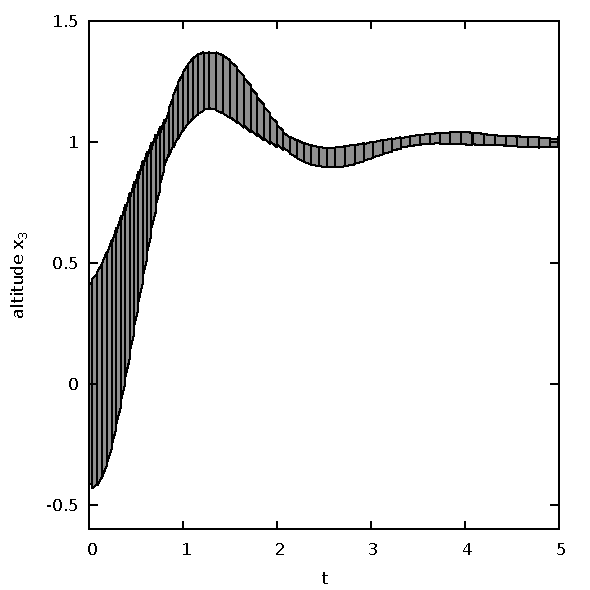
\includegraphics[width=5.5cm, height=5.5cm]{results_Isabelle/out_quadrot.pdf}
  \label{fig:quadrotor:isabelle}}
\subfigure[SymReach.] 
	  {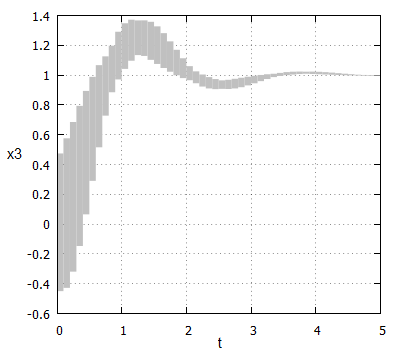
\includegraphics[width=5.5cm, height=5.5cm]{results_SymReach/quadrotor.png}
  \label{fig:quadrotor:SymReach}}

\caption{Reachable set overapproximations for the quadrotor model.}
\label{fig:quadrotor}
\end{figure}


\begin{table}[t]
	\setlength{\tabcolsep}{4pt}
	\renewcommand{\arraystretch}{1.2}
	\centering
	\caption{Results of the quadrotor model. Details of the platforms are described in Section~\ref{sec:machines}.}
	\begin{tabular}[c]{lccc}
	\hline
		 \textbf{tool} & \textbf{computation time in [s]} & \textbf{language} & \textbf{machine} \\
		 \hline
         CORA & $5.2$ & MATLAB & M$_{\text{CORA}}$ \\
         CORA/SX & $1.5$ & C++ & M$_{\text{SpaceEx}}$ \\
         Flow* & $5.9$ & C++ & M$_{\text{Flow*}}$ \\
         Isabelle/HOL & 30 & SML & M$_{\text{Isabelle}}$ \\
         SymReach & 2.96 & C++ & M$_{\text{SymReach}}$ \\
		 \hline
	\end{tabular}
	\label{tab:compTimes:quadrotor}
\end{table}


\subsubsection{Results}


The results of the reachability computation for the quadrotor model are given in Figure~\ref{fig:quadrotor} and Table~\ref{tab:compTimes:quadrotor}. We give the tool settings below.

\paragraph{Setting for CORA.}
CORA uses the step size $0.1$ and the zonotope order $50$. The computation is carried out using the approach in \cite{Althoff2008c}, which conservatively linearizes the system dynamics for each consecutive time interval by adding the linearization error as an uncertain input. The linearization error is obtained using the Lagrange remainder, which are evaluated via interval arithmetic. This results in many function calls (especially for this example), whose overhead has been reduced since MATLAB R2015b. So the execution time for the quadrotor benchmark depends significantly on the MATLAB version (more than twice as fast since R2015b).

\paragraph{Setting for CORA/SX.}
CORA/SX uses the step size $0.05$ and the zonotope order $50$. Note that the plot of CORA/SX in Fig.\;\ref{fig:quadrotor:corasx} does not have a staircaise form like CORA and SymReach, because time needs to be added as a state variable for CORA/SX to be able plot over time.

\paragraph{Setting for Flow*.}
Flow* uses the step size $0.025$, the TM order $4$, the cutoff threshold $10^{-6}$ and the precision $53$ for floating-point numbers. The TM flowpipe remainders are kept symbolically every $20$ steps. All floating-point roundoff errors are included in the overapproximation. Figure~\ref{fig:quadrotor:flow*} illustrates the interval overapproixmations for the flowpipes. To better evaluate the approximation error, we provide the maximum overapproximation error of the last flowpipe which is below $0.0003103$. Besides, the altitude at $t=5$ is below $1$ according to the computed flowpipes.

\paragraph{Setting for Isabelle/HOL.}
Maximum Zonotope order is set to $25$. Reachability analysis is carried out with an (absolute and relative) error tolerance of $2^{-10}$.

\paragraph{Setting for SymReach.}
Step size is set to $0.1$, zonotope order limited to $5$, $L_{max} = 0.05$. 



\clearpage

\subsection{Space Rendezvous Benchmark}
\label{sec:spacerendezvous}

\subsubsection{Model}

Spacecraft rendezvous is a perfect use case for formal verification of hybrid systems with nonlinear dynamics since mission failure can cost lives and is extremely expensive. This benchmark is taken from \cite{Chan2017a}. A version of this benchmark with linearized dynamics is verified in the ARCH-COMP category \textit{Continuous and Hybrid Systems with Linear Continuous Dynamics}. The nonlinear dynamic equations describe the two-dimensional, planar motion of the spacecraft on an orbital plane towards a space station:

\[
\left\{
\begin{array}{lcl}
 \dot{x} & = & v_x \\
 \dot{y} & = & v_y \\
 \dot{v_x} & = & n^2 x + 2n v_y + \frac{\mu}{r^2} - \frac{\mu}{r_c^3} (r + x) + \frac{u_x}{m_c} \\
 \dot{v_y} & = & n^2 y - 2n v_x - \frac{\mu}{r_c^3} y + \frac{u_y}{m_c}\\
\end{array}
\right.
\]
The model consists of position (relative to the target) $x, y$ [m], time $t$ [min], as well as horizontal and vertical velocity $v_x, v_y$ [m / min]. The parameters are $\mu = 3.986 \times 10^{14} \times 60^2$ [m$^3$ / min$^2$], $r = 42164 \times 10^3$ [m], $m_c = 500$ [kg], $n = \sqrt{\frac{\mu}{r^3}}$ and $r_c = \sqrt{(r+x)^2 + y^2}$.

\newcommand{\vecT}[1]{\begin{pmatrix}#1\end{pmatrix}^T}
\newcommand{\psmat}[1]{\begin{psmallmatrix}#1\end{psmallmatrix}}

The hybrid nature of this benchmark origins from a switched controller. In particular, the modes are \textit{approaching}
($x \in [-1000, -100]$ [m]), \textit{rendezvous attempt} ($x \ge -100$ [m]), and \textit{aborting} (time $t \ge 120$ [min]). The linear feedback controllers for the different modes are defined as $\psmat{u_x \\ u_y} = K_1 \underline{x}$ for mode \textit{approaching}, and $\psmat{u_x \\ u_y} = K_2 \underline{x}$ for mode \textit{rendezvous attempt}, where $\underline{x} =
\vecT{x & y & v_x & v_y}$ is the vector of system states. The feedback matrices $K_i$ were determined with an LQR-approach applied to the linearized system dynamics, which resulted in the following numerical values:

\begin{align*}
	& K_1 = \begin{pmatrix} -28.8287 & 0.1005 & -1449.9754 &   0.0046 \\
  -0.087 & -33.2562 & 0.00462 & -1451.5013 \end{pmatrix} \\
    & ~ \\
    & K_2 = \begin{pmatrix} -288.0288 & 0.1312 & -9614.9898 & 0 \\
  -0.1312 & -288 & 0 & -9614.9883 \end{pmatrix}
\end{align*}
In the mode \textit{aborting} the system is uncontrolled $\psmat{u_x \\ u_y} = \psmat{0 \\ 0}$. 


\subsubsection{Specification}

The spacecraft starts from the initial set $x \in [-925,-875]$ [m], $y \in [-425,-375]$ [m], $v_x = 0$ [m/min] and $v_y = 0$ [m/min]. For the considered time horizon of $t \in [0,200]$ [min], the following specifications have to be satisfied:

\begin{itemize}
\item \textbf{Line-of-sight:} In mode \textit{rendezvous attempt}, the spacecraft has to stay \\
inside line-of-sight cone $\mathcal{L} = \{ \psmat{x \\ y} \mid (x \geq -100) \land (y \geq x \tan(30^\circ)) \land (-y \geq x \tan(30^\circ))\}$.
%
\item \textbf{Collision avoidance:} In mode \textit{aborting}, the spacecraft has to avoid a collision with the target, which is modeled as a box $\mathcal{B}$ with 0.2m edge length and the center placed at the origin.
%
\item \textbf{Velocity constraint:} In mode \textit{rendezvous attempt}, the absolute velocity has to stay below $3.3$ [m/min]: $\sqrt{v_x^2 + v_y^2}\leq 3.3$ [m/min].
\end{itemize}

\paragraph{Remark on velocity constraint} In the original benchmark~\cite{Chan2017a}, the constraint on the velocity was set to 0.05 m/s, but it can be shown (by a counterexample) that this constraint cannot be satisfied. We therefore use (just like the ARCH-COMP category \textit{Continuous and Hybrid Systems with Linear Continuous Dynamics}) the relaxed constraint 0.055 [m/s] = 3.3 [m/min].

% This property can be proved for the linearized system . We can show that using the same controller for the nonlinear dynamics results in exceeding this constraint (see figure~\ref{fig:spacecraft_vel}).
% \end{itemize}
% \begin{figure}[ht!b]
% \centering
% \includegraphics[width=0.45\columnwidth, height=5.5cm]{results_Isabelle/out_space_vel.pdf}
%   \label{fig:spacecraft_vec}
% \caption{Reachable set of the spacecraft velocity proves that
% the velocity constraint is exceeded.}
% \label{fig:spacecraft_vel}
% \end{figure}


\subsubsection{Results}

The results of the reachability computation for the spacecraft rendezvous model are given in Figure~\ref{fig:spacecraft} and Table~\ref{tab:compTimes:spacecraft}, with the tool settings below.

\begin{table}[t]
	\setlength{\tabcolsep}{4pt}
	\renewcommand{\arraystretch}{1.2}
	\centering
	\caption{Results of the spacecraft rendezvous model. Details of the platforms are described in Section~\ref{sec:machines}.}
	\begin{tabular}[c]{lccc}
	\hline
		 \textbf{tool} & \textbf{computation time in [s]} & \textbf{language} & \textbf{machine} \\
		 \hline
         CORA & $14.8$ & MATLAB & M$_{\text{CORA}}$ \\
         {C2E2} & {$29.18$} & {C++} & {M$_{\text{C2E2}}$} \\
         Flow* & $18.7$ & C++ & M$_{\text{Flow*}}$ \\
         Isabelle/HOL & 395 & SML & M$_{\text{Isabelle}}$ \\
		 \hline
	\end{tabular}
	\label{tab:compTimes:spacecraft}
\end{table}

\begin{figure}[t]
\centering
\subfigure[CORA.] 
{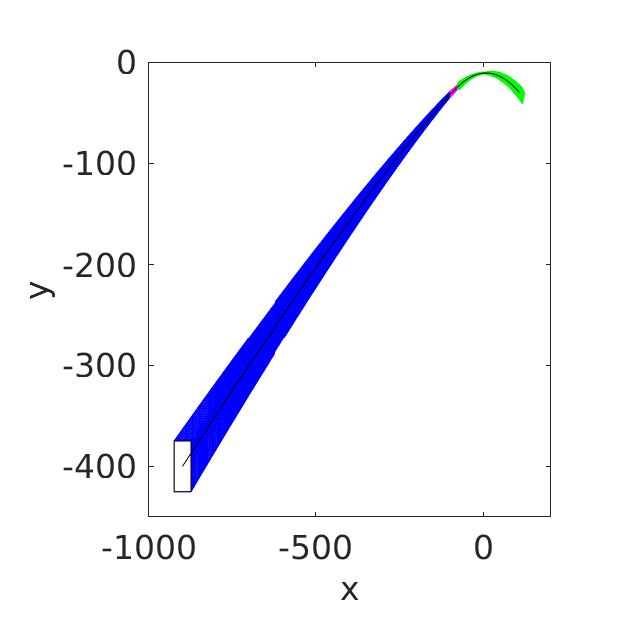
\includegraphics[width=5.5cm, height=5.5cm]{results_CORA/spacecraftNonlin_04June2018.eps}
  \label{fig:spacecraft:cora}}
  %\hspace{0.2in}
\subfigure[C2E2.] 
	  {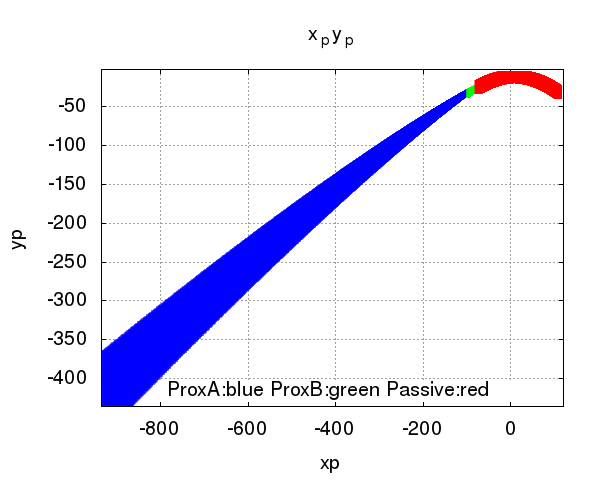
\includegraphics[width=5.5cm, height=5.5cm]{results_C2E2/nln_4d_pass.png}
  \label{fig:spacecraft:C2E2}}
  \hspace{0.2in}

\subfigure[Flow*.] 
	  {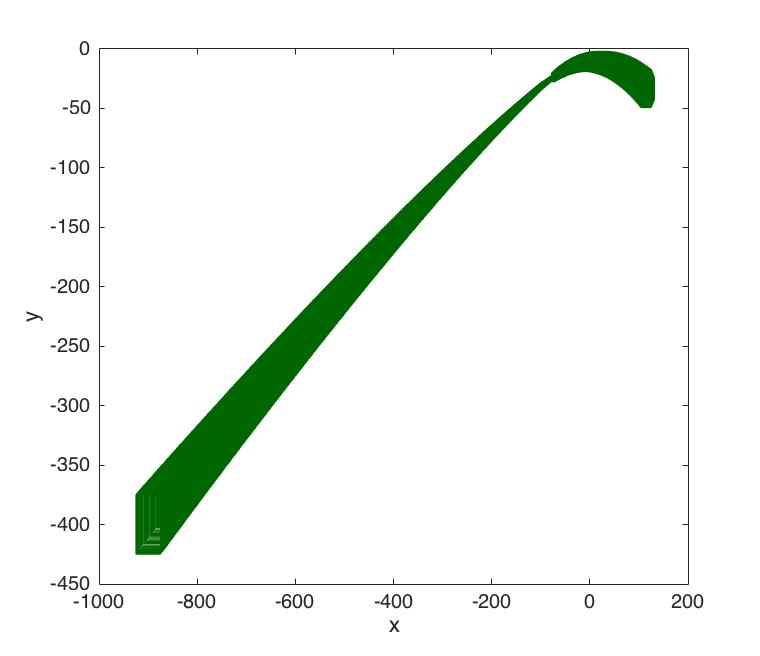
\includegraphics[width=5.5cm, height=5.5cm]{results_flowstar/Space_Rendezvous.png}
  \label{fig:spacecraft:flowstar}}
  \hspace{0.2in}
\subfigure[Isabelle/HOL.] 
	  {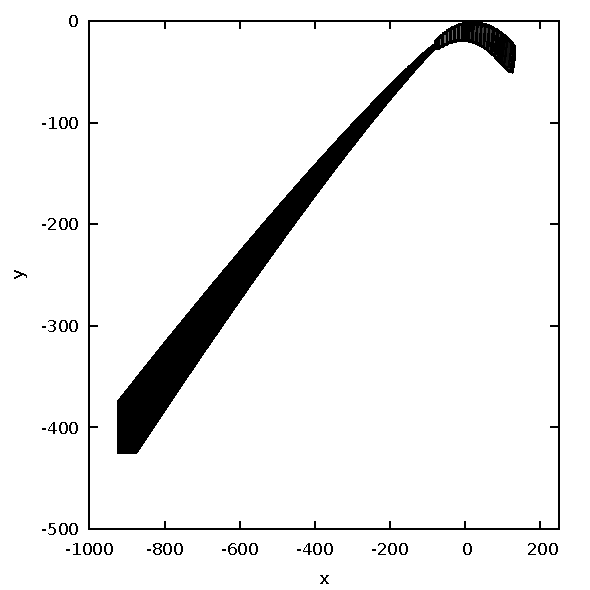
\includegraphics[width=5.5cm, height=5.5cm]{results_Isabelle/out_space.pdf}
  \label{fig:spacecraft:isabelle}}
  \hspace{0.2in}
\caption{Reachable set of the spacecraft position in the $x$-$y$-plane.
CORA shows simulations in black. CORA and C2E2 use different colors to encode different modes of the hybrid system. C2E2 with abortion mode linearized.}
\label{fig:spacecraft}
\end{figure}


\paragraph{Setting for CORA.}
CORA was run with a time step size of $0.2$ [min] for the modes \textit{approaching} and \textit{aborting}, and with a time step size of $0.05$ [min] for mode \textit{rendezvous attempt}. The intersections with the guard sets were calculated with the method of Girard, which was introduced in \cite{Girard2008}. In order to find suitable orthogonal directions, the last zonotope that did not intersect the guard set is projected onto the hyperplane that represents the guard set. Then, Principal Component Analysis is applied to the generators of the projected zonotope.

\paragraph{Setting for C2E2.} C2E2 can verify this model when the abortion mode is linearized. Since C2E2 cannot take nonlinear unsafe set specifications, the thrust constraint is safely underapproximated by an octagon. Moreover, since C2E2 cannot handle unsafe set specifications with logical conjunction, each constraint is checked separately and the sum of run time for each individual constraint represents the total run time for verifying the model. The time step used to solve the model is 0.1 and the K value used is 2000. Note that the result for C2E2 is not optimal since C2E2 is currently been updated.

\paragraph{Setting for Flow*.}
The model can be directly verified by Flow* with the following setting for parameters: the TM order is fixed by $5$, the stepsize is adaptively selected in the range from $0.001$ to $0.5$, the remainder estimation is the interval $[-10^{-3},10^{-3}]$ in all dimensions, and the cutoff threshold is $10^{-6}$. Besides, we use the precision $100$. We simply aggregate the intersections after each jump by a box instead of a parallelotope which is more time-costly to compute but more accurate, since it is already sufficient to prove the property.

\paragraph{Setting for Isabelle/HOL.}
Isabelle/HOL does not support hybrid systems automatically.
One can, however, compute the reachable sets for each mode seperately. The intersection with the guard set is computed with the method of Girard~\cite{Girard2008}, simply using axis-aligned orthogonal directions, which results in box enclosures. We verify that the transition to mode \emph{rendezvous attempt} occurs at
$t \in [108.66, 111.71]$,
$x = -100$,
$y \in [-35.04, -28.43]$,
$v_x \in [1.99365, 2.00644]$,
$v_y \in [0.6489, 0.8130]$. Starting from this box, the transition to mode \emph{aborting} occurs at
$t = 120$,
$x \in [-78.02, 71,20]$,
$y \in [-27.34, -20.23]$,
$v_x \in [2.135, 2.341]$,
$v_y \in [0.603, 0.825]$. From there we compute the reachable set until time $t = 200$, which satisfies $y < -1$ [m].
In those computations, maximum zonotope order is set to $50$ and we use absolute and relative error tolerance of $2^{-10}$.

%------------------------------------------------------------------------------

\iffalse
\subsection{Artificial Pancreas}
\label{sec:artificialpancreas}

\subsubsection{Model}

The artificial pancreas benchmark model was introduced in \cite{Chen2017}. It is a hybrid system with nonlinear dynamics. The benchmark models the scenario of an artificial pancreas that automates the delivery of insulin to patients with type-1 diabetes. For the test case, it is assumed that the patient consumes a meal at time $t=0$. It then has to be guaranteed that the controller is able to keep the blood glucose levels at amounts that are not live threatening for the patient. The system states of the benchmark as defined in \cite{Chen2017} (Tab. 2) are the insulin concentration in the remote chamber $X$, the subcutaneous insulin in chamber \#1 $I_{sc1}$ and in chamber \#2 $I_{sc2}$, the glucose concentration in rapidly equilibriating tissues $G_t$, the glucose concentration in plasma $G_p$, the portal vein insulin concentration $I_l$, the insulin in plasma $I_p$, the insulin concentration in chamber \#1 $I_1$, the delayed insulin from chamber \#1 $I_d$ and the subcutaneous glucose concentration $G_s$. 


The differential equations for the artificial pancreas model are given according to \cite{Chen2017}:

\[
\left\{
\begin{array}{lcl}
\dot{X} & = & -0.0278X + 0.0278(18.2129 I_p - 100.25)\\
\dot{I}_{sc1} & = &  -0.0171 * I_{sc1} + 0.97751710655*u_I(t) \\
\dot{I}_{sc2} & = & 0.0152 I_{sc1} - 0.0078 I_{sc2} \\
\dot{G}_t & = & -0.0039 (3.2267+0.0313X) G_t ( 1 - 0.0026 G_t + (2.5097 \times 10^{-6}) G_t^2) \\
& & + 0.0581 G_p - 0.0871 G_t \\
\dot{G}_p & = & 4.7314 - 0.0047 G_p - 0.0121 I_d - 0.0581 G_p + 0.0871 G_t + u_m(t) \\
\dot{I}_l & = & -0.4219 I_l + 0.2250 I_p \\
\dot{I}_p & = & -0.3150 I_p + 0.1545 I_l + 0.0019 I_{sc1} + 0.0078 I_{sc2} \\
\dot{I}_1 & = & -0.0046 ( I_1 - 18.2129 I_p) \\
\dot{I}_d & = & -0.0046 (I_d - I_1 ) \\
\dot{G}_s & = & 0.1 ( 0.5221 G_p - G_s) \\
\end{array}
\right.
\]

The system input $u_m(t) = D u_{m,1}(t)$ is defined by the meal absorption model according to [\cite{Chen2017}, eq. (2)]:

\[
u_{m,1}(t) = \left\{
\begin{array}{lcl}
0 & & t \leq 0\\
1.141 \times 10^{-4} t^2 + 6.134 \times 10^{-6} t & & 0 \leq t \leq 30 \\
5.25 \times 10^{-5} t^2 - 7.468 \times 10^{-3} t + 0.281 & & 30 < t \leq 80 \\
1.245 \times 10^{-7} t^2 - 9.112 \times 10^{-5} t + 2.648 \times 10^{-2} & & 80 < t \leq 360 \\
-6.307 \times 10^{-5} t^2 + 0.0483 t -9.190 & & 360 < t \leq 400 \\
3.553 \times 10^{-6} t^2 - 3.423 \times 10^{-3} t + 0.824 & & 400 < t \leq 500 \\
1.113 \times 10^{-8} t^2 - 1.482 \times 10^{-5} t + 4.9 \times 10^{-3} & & 500 < t \leq 720 \\
0 & & t \geq 720
\end{array}
\right.,
\]
and by the amount of Carbohydrates $D \in [70,80]$ in the meal consumed by the patient. The second system input $u_I(t) = I$ is given by the controller depicted in Fig.~\ref{fig:pancreasController}. One of the main challenges for this benchmark model is the efficient computation of guard intersections in a high dimensional space. 

\begin{figure}[htb]
    \centering	
    \scriptsize
	
      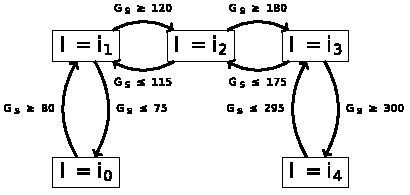
\includegraphics[width=0.6\columnwidth]{./figures/pancreasController.pdf}
      \caption{Control law $u_I(t) = I$ for the artificial pancreas benchmark. The discrete control inputs are defined as $i_0 = 0$, $i_1 = 0.1$, $i_2 = 0.2$, $i_3 = 0.5$ and $i_4 = 1.4$.}
      \label{fig:pancreasController}
\end{figure}


\subsubsection{Specification}

We consider the initial set $X = 0$, $I_{sc1} = 72.42$, $I_{sc2}=141.15$, $G_t=162.45$, $G_p \in [229.824, 268.128]$, $I_l=3.2$, $I_p=5.5$, $I_1 = 100.25$, $I_d=100.25$ and $G_s \in [120,160]$. The amount of Carbohydrates $D \in [70,80]$ in the consumed meal represents an uncertain system input. The unsafe set is $G_s \geq 350$. Further, it is required that $(G_s \leq 300) \land (G_s \geq 250)$ at time $t = 720$. The considered time horizon for the verification is $t \in [0, 720]$. 

\subsubsection{Results}

The results of the reachability computation for the artificial pancreas model are given in Figure~\ref{fig:pancreas} and Table~\ref{tab:compTimes:pancreas}. We give the settings for CORA and Flow* as below.

\begin{table}[h]
	\setlength{\tabcolsep}{4pt}
	\renewcommand{\arraystretch}{1.2}
	\centering
	\caption{Results of the artificial pancreas model. Details of the platforms are described in Section~\ref{sec:machines}.}
	\begin{tabular}[c]{lccc}
	\hline
		 \textbf{tool} & \textbf{computation time in [s]} & \textbf{language} & \textbf{machine} \\
		 \hline
         CORA & $39$ & MATLAB & M$_{\text{CORA}}$ \\
         Flow* & x & C++ & M$_{\text{Flow*}}$ \\
         Isabelle/HOL & x & SML & M$_{\text{Isabelle}}$ \\
		 \hline
	\end{tabular}
	\label{tab:compTimes:pancreas}
\end{table}

\begin{figure}[ht!b]
\centering
\subfigure[CORA.] 
	  {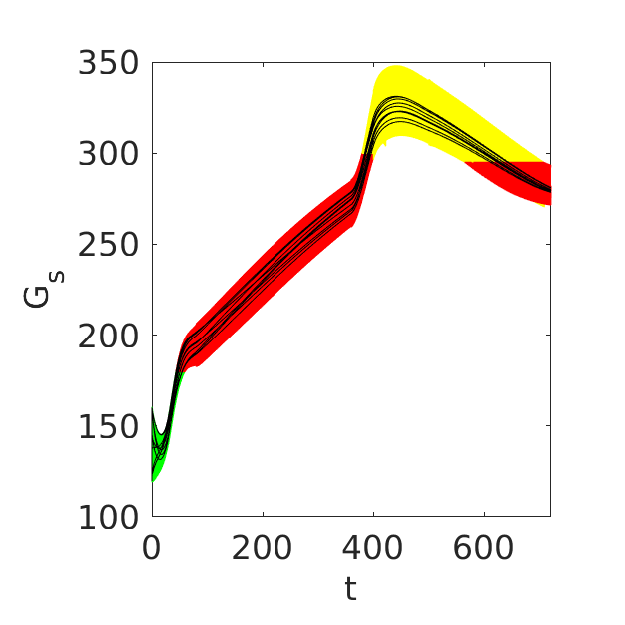
\includegraphics[width=0.45\columnwidth, height=5.5cm]{results_CORA/pancreas_30May2018.eps}
  \label{fig:pancreas:cora}}
  \hspace{0.2in}
\caption{Reachable set of the glucose concentration $G_s$ plotted over time. Simulations are shown in black. The different colors encode different invariant sets of the hybrid system.}
\label{fig:pancreas}
\end{figure}


\paragraph{Setting for CORA.}

CORA uses the step size $0.5$ and the zonotope order $4$. The computation within the invariant sets is carried out using the approach in \cite{Althoff2008c}, which conservatively linearizes the system dynamics for each consecutive time interval by adding the linearization error as an uncertain input. For the calculation of intersections with the guard intersections the approach from \cite{Girard2008} is used. In order to find suitable orthogonal directions, the last zonotope that did not intersect the guard set is projected onto the hyperplane that represents the guard set. Then, Principal Component Analysis is applied to the generators of the projected zonotope.

\paragraph{Setting for Flow*.}





\subsection{Plots}

\subsubsection{Van der Pol Oscillator}

\subsubsection{Laub-Loomis Model}

\textbf{Isabelle Notes:} Reachability Analysis for $W = 0.1$ after splitting the initial set along $x_1$, $x_2$, and $x_3$.

\begin{figure}[ht!b]
\centering
\subfigure[CORA.] 
	  {\includegraphics[width=0.45\columnwidth]{results_CORA/LaubLoomis_30Mar2017.eps}
  \label{fig:laubloomis_easy:cora}}
  \hspace{0.2in}
\subfigure[Isabelle.] 
	  {\includegraphics[width=0.45\columnwidth]{results_Isabelle/laub_time_easy.pdf}
  \label{fig:laubloomis_easy:isabelle}}
\caption{Reachable sets (W=0.01).}
\label{fig:laubloomis}
\end{figure}







\subsection{Quadrotor Model}




\subsection{Computation Times}

The computation times of various tools for the van der Pol benchmark are listed in Tab.~\ref{tab:compTimes:vanderpol}.


\begin{table}[h]
	\setlength{\tabcolsep}{4pt}
	\renewcommand{\arraystretch}{1.2}
	\centering
	\caption{Computation Times of the van der Pol Benchmark.}
	\begin{tabular}[c]{lccccc}
	\hline
		 & \multicolumn{3}{c}{\textbf{computation time in [s]}} & \multicolumn{2}{c}{\textbf{platform}} \\ \cmidrule(l){2-4} \cmidrule(l){5-6}
		 \textbf{tool} & \textbf{van der Pol} & \textbf{Laub ($W=0.01$)} & \textbf{Laub ($W=0.1$)} & $\textbf{language}$ & $\textbf{machine (see  Sec.~\ref{sec:machines})}$ \\ \hline
         CORA & $9$ & $3$ & $63$ & MATLAB & M$_{CORA}$ \\
         Flow* & $2$ & $8$ & $18$ & C++ & M$_{\text{Flow*}}$ \\
         Isabelle & $3$ & $60$ & $2700$ & SML & M$_{Isabelle}$ \\
		 \hline
	\end{tabular}
	\label{tab:compTimes:vanderpol}
\end{table}
\fi

%------------------------------------------------------------------------------
%\section{Discussion}
%\label{sect:discussion}


%------------------------------------------------------------------------------
\section{Conclusion and Outlook}
\label{sect:conclusion}

% From the results of the competition on nonlinear systems, we can see that the techniques handling nonlinear dynamics often require more user-specified parameters than those for linear dynamics. all of the tools have their advantages on some examples, and the applicability of a tool to one example is usually quite sensitive to the computational setting in use. Therefore, it could be a promising direction for coming up with new techniques to find proper settings for a tool and optimize its performance for a given computation task.

% In the next year, we hope that more tools could join the friendly competition and we will also collect more benchmarks which are not only continuous but also hybrid. We will also try to expose the advantages of different tools by examples. The reports of other categories can be found in the proceedings and on the ARCH website:  \href{http://cps-vo.org/group/ARCH}{cps-vo.org/group/ARCH}.
In last year's competition~\cite{ARCH_COMP17}, we promised to include hybrid benchmarks and hoped that more tools would join the competition.
Indeed, three new tools (C2E2, CORA/SX, SymReach) participated. Hybrid dynamics is included in the new benchmark Space Rendezvous (section~\ref{sec:spacerendezvous}). A linearized version of the Space Rendezvous benchmark was used in the ARCH-COMP category \textit{Continuous and Hybrid Systems with Linear Continuous Dynamics}.

Triggered by the participation in this competition, individual tools made progress and can now solve benchmarks that were previously out of reach:
\begin{itemize}
\item This is the first time \textbf{C2E2} participates in the competition. The results for C2E2 are not optimal because a new version of C2E2 is about to be released with the experience gained during the competition. 
\item The tool \textbf{Flow*} has been improved in the following aspects since the last competition. Firstly, we optimized some interval computation procedure to overall improve the performance. Secondly, the C++ API of the tool is under development, we currently exposed all functions for handling LTI and LTV dynamics as well as linear constraints. It provides not only a much more flexible way to handle different systems, but also a possibility to cooperate with program analysis tools to handle more complex controlled systems. Besides, Flow* will also support the formal verification of continuous systems with neural network controllers.
\item Compared to last year, \textbf{Isabelle/HOL} includes affine arithmetic approximations for some transcendental functions ($\sin,\cos,\exp,\sqrt{\phantom{x}}$) and can therefore now solve the Quadrotor benchmark.
\end{itemize}

A direct outcome of this competition is that one has a means of comparing the available tools for nonlinear reachability analysis. An indirect outcome is that individual tools made progress and more tools and algorithms are available.
The direct and indirect outcomes of this competition serve the whole community interested in developing and applying tools for reachability analysis of nonlinear systems: We can claim that this competition helps to advance and promote the state-of-the-art of tools for nonlinear reachability analysis.

%------------------------------------------------------------------------------
\section{Acknowledgments}
\label{sect:acks}


The authors gratefully acknowledge financial support by the European Commission project UnCoVerCPS under grant number 643921.


\appendix
\section{Specification of Used Machines} \label{sec:machines}

\subsection{\texorpdfstring{M$_{\text{CORA}}$}{M-CORA}} \label{sec:machine:CORA}

\begin{itemize}
    \item Processor: Intel Core i7-7820HQ CPU @ 2.90GHz x 4 
    \item Memory: 32 GB
    \item Average CPU Mark on \url{www.cpubenchmark.net}: 9409 (full), 2070 (single thread)
\end{itemize}

\subsection{\texorpdfstring{M$_{C2E2}$}{M-C2E2}} \label{sec:machine:C2E2}
\begin{itemize}
	\item Processor: Intel Core i5-3470 CPU @ 3.20GHz x 4 
    \item Memory: 8 GB
    \item Average CPU Mark on \url{www.cpubenchmark.net}: 6680 (full), 1915 (single thread)
\end{itemize}

\subsection{\texorpdfstring{M$_{\text{Flow*}}$}{M-Flow*}} \label{sec:machine:flowstar}
Virtual machine on VMware Workstation 11 with a single core CPU and 4.0 GB memory. The operating systems is Ubuntu 16.04 LTS. The physical CPU is given as below.
\begin{itemize}
 \item Processor: Intel Xeon E3-1245 V3 @ 3.4GHz x 4
 \item Average CPU Mark on \url{www.cpubenchmark.net}: 9545 (full), 2155 (single thread)
\end{itemize}

\subsection{\texorpdfstring{M$_{\text{Isabelle}}$}{M-Isabelle}} \label{sec:machine:isabelle}
\begin{itemize}
 \item Processor: Intel Core i7-8750H CPU @ 2.20GHz x 6
 \item Memory: 16 GB 2666 MHz DDR4
 \item Average CPU Mark on \url{www.cpubenchmark.net}: 12,516 (full), 2368 (single thread)
\end{itemize}

\subsection{\texorpdfstring{M$_\mathit{SpaceEx}$}{M-SpaceEx}} \label{sec:machine:spaceex}
\begin{itemize}
	\item Processor: Intel Core i7-7920HQ CPU @ 3.1GHz x 4
    \item Memory: 16 GB
    \item Average CPU Mark on \url{www.cpubenchmark.net}: 10230 (full), 2161 (single thread)
\end{itemize}

\subsection{\texorpdfstring{M$_{\text{SymReach}}$}{M-SymReach}} \label{sec:machine:SymReach}
\begin{itemize}
 \item Processor: Intel Core Duo T2250 CPU @ 1.73GHz x 2
 \item Memory: 1.5 GB
 \item Average CPU Mark on \url{www.cpubenchmark.net}: 758 (full), 547 (single thread)
\end{itemize}


\bibliographystyle{plain}
%\bibliographystyle{alpha}
%\bibliographystyle{unsrt}
%\bibliographystyle{abbrv}
\bibliography{bib/chen,bib/althoff_other,bib/althoff_own,bib/frehse,bib/immler,bib/c2e2,bib/SymReach}

\end{document}
